\chapter{Bremsstrahlung}
\label{cha:bremsstrahlung}
\index{bremsstrahlung}
Bremsstrahlung or braking radiation is the radiation that the charged
particle emits while being accelerated in the electric field of
another particle.  Because the amount of radiation produced is
proportional to the square of the acceleration, the less massive
particle generally dominates the emission.  Typically, we are talking
about an electron and an ion, so the mass ratio is greater than 1,800
to one.

Why is it called bremsstrahlung?  X-rays were first produced in the
laboratory by accelerating electrons along a strong electric field (a
typical potential difference of 10kV) from an anode to a cathode in
vacuum.  When the electrons hit the thick metal cathode and stop
(brake), they emit cathode rays or X-rays.

\section{The Physics of Bremsstrahlung}
\label{sec:phys-bremsstr}

If we ignore the effect of radiation reaction of the trajectory of the
charged particle, we can solve for its path exactly (at least in the
classical limit) and then use the formulae for the radiation field
that we derived a few weeks back.   You can check out the Padmanabhan
text if you would like to see an exact treatment.

\paragraph{Something to think about.}  What is the exact classical 
trajectory of the charged particle?  

We will approximate the exact trajectories shown in the left-hand
panel of Fig.~1 by a simple straight line trajectory in which the
acceleration of the particle lies mainly normal to the direction of the
particle's motion.
{
\begin{figure}
\centering
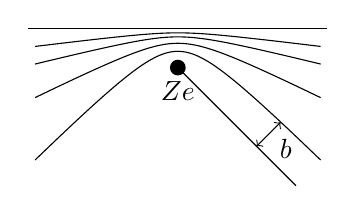
\begin{tikzpicture}
\draw plot [domain=-2:2,smooth] ({(exp(-\x)-exp(\x))/4}, {(-exp(\x)-exp(-\x))/4});
\draw plot [domain=-2:2,smooth] ({(exp(-\x)-exp(\x))/4}, {(-exp(\x)-exp(-\x))/8+sqrt(1/4+1/16)-sqrt(0.5)});
\draw plot [domain=-2:2,smooth] ({(exp(-\x)-exp(\x))/4}, {(-exp(\x)-exp(-\x))/16+sqrt(1/4+1/64)-sqrt(0.5)});
\draw plot [domain=-2:2,smooth] ({(exp(-\x)-exp(\x))/4}, {(-exp(\x)-exp(-\x))/32+sqrt(1/4+1/256)-sqrt(0.5)});
\draw (-1.9,-0.2071067812) -- (1.9,-0.2071067812) ;
\fill (0,-0.707) circle (0.1) ;
\draw (0,-0.707) -- ++(1.5,-1.5);
\draw [<->] (0,-0.707) ++(1,-1) -- ++(0.305,0.305) ;
\draw (0,-1) node {$Ze$} ;
\draw  (0,-0.707) ++(1.2,-1.2) ++(0.1725,0.1725) node {$b$};
\end{tikzpicture}
\begin{tikzpicture}
\draw [->] (0,0) -- (4,0) ;
\draw (4.2,0.2) node {$\vec v$};
\draw [dashed] (0.5,0) -- (0.5,-2) ;
\draw (0.1,-2) node {$Ze$} ;
\draw (0.3,-0.5) node {$b$} ;
\draw [->] (0.5,-2) -- (3,0) ;
\draw (3,-0.5) node {$\vec R$} ;
\fill (3,0) circle (0.1) ;
\fill (0.5,-2) circle (0.1) ;
\draw (3,0.2) node {$e$} ;
\end{tikzpicture}
\caption{Bremsstrahlung.  The left panel gives the exact trajectory
  excluding radiation reaction, and the right panel shows how we will
  approximate the trajectory}

\end{figure}
}

\paragraph{Something to think about.}  When does the straight line 
approximation fail?

We will also use the dipole approximation, so ${\bf d} = -e {\bf R}$
where ${\bf R}$ is the position of the particle.  By taking the time
derivative on both sides twice we find,
\begin{equation}
\ddot{\bf d} = -e\dot{\bf v}
\label{eq:326}
\end{equation}
Ultimately we will be interested in the Fourier transform of the
radiation field to understand the spectrum so we have,
\begin{equation}
-\omega^2 \hat{\bf d}(\omega) = -\frac{e}{2\pi} \int_{-\infty}^\infty
\dot{\bf v} e^{i\omega t} dt.
\label{eq:327}
\end{equation}
Most of the acceleration of the particle occurs during a short time in
which $R\sim b$.  This {\it collision time} is approximately
\begin{equation}
\tau = \frac{b}{v}
\label{eq:328}
\end{equation}
so the bulk of the contribution to the integral happens for $-\tau \lesssim t
\lesssim \tau$.  If $\omega \tau \gg\ 1$, the integrand will oscillate 
rapidly so the integral will be small.  On the other hand if
$\omega\tau \ll 1$ the exponential is essentially unity so
\begin{equation}
\hat{\bf d}(\omega) \sim \left \{ 
\begin{array}{cl}
\frac{e}{2\pi\omega^2} {\bf \Delta v}, &\omega \tau \ll\ 1 \\
 0, & \omega\tau \gg 1
\end{array}
\right .
\label{eq:329}
\end{equation}
where $\bf{\Delta v}$ is the change of velocity during the collision.

The energy spectrum is given by
\begin{equation}
\dd{W}{\omega} = \frac{8\pi \omega^4}{3c^3} \left | \hat{d}(\omega)
\right |^2 = 
\left \{
\begin{array}{cl}
\frac{2 e^2}{3\pi c^3} \left | {\bf \Delta v} \right |^2, &\omega \tau \ll\ 1 \\
 0, & \omega\tau \gg 1
\end{array}
\right .
\label{eq:330}
\end{equation}
Let's estimate the value of $\Delta v$,
\begin{equation}
\Delta v =  \int_{-\infty}^\infty \frac{b}{R}
\frac{1}{m} \frac{Ze^2}{R^2} dt = \frac{Z e^2}{m} 
\int_{-\infty}^\infty \frac{b}{\left ( b^2 + v^2 t^2 \right )^{3/2}} dt
= \frac{2 Z e^2}{m b v}
\label{eq:331}
\end{equation}
so we can estimate the emission from a single collision 
\begin{equation}
\dd{W(b)}{\omega} = 
\left \{
\begin{array}{cl}
\frac{8 Z^2 e^6}{3\pi c^3 m^2 v^2 b^2}, & b \ll v/\omega \\
 0, & b \gg v/\omega
\end{array}
\right .
\label{eq:332}
\end{equation}
We would like to integrate over all impact parameters.  We know that
for a particular frequency, $\omega$, the contribution to the spectrum
vanishes for $b \gg\ v/\omega$.   Let's assume that
there is a mininum value of the impact parameter $b_\rmscr{min}$ below
which our analysis fails.  Looking at the left-hand panel of Fig.~1,
you may be able to figure out when this is the case, so we 
have
\begin{eqnarray}
\frac{d W}{d\omega dV dt} &=& n_e n_i 2\pi v \int_{b_\rmscr{min}}^{b_\rmscr{max}}
\frac{8 Z^2 e^6}{3\pi c^3 m^2 v^2 b^2} b d b
 \\ 
&=& \frac{16 e^6}{3 c^3 m^2 v} n_e n_i Z^2
\int_{b_\rmscr{min}}^{b_\rmscr{max}} \frac{db}{b}\\
&=&
\frac{16 e^6}{3 c^3 m^2 v} n_e n_i Z^2 \ln \left
(\frac{b_\rmscr{max}}{b_\rmscr{min}} \right )
\label{eq:333}
\end{eqnarray}
We can see that our particular choice of the minimum and maximum
impact parameters is not particularly important because they enter
logarthimically.  We can take
\begin{equation}
b_\rmscr{max} \equiv \frac{v}{\omega}.
\end{equation}
There are two ways to get a value of $b_\rmscr{min}$.  First is to
estimate at what impact parameter does the trajectory strongly differ
from a straight line, so $\Delta v \sim v$, we get
\begin{equation}
v \sim \Delta v(b_\rmscr{min}^{(1)}) = 
 \frac{2 Z e^2}{m b_\rmscr{min}^{(1)} v} \rightarrow b_\rmscr{min}^{(1)}
  \sim \frac{2 Z e^2}{m v^2}.
\label{eq:334}
\end{equation}
We could have gotten this same value if we had compared the initial
kinetic energy of the particle with its potential energy at point of
closest approach.  The standard value is slightly different
\begin{equation}
 b_\rmscr{min}^{(1)} 
  = \frac{4 Z e^2}{\pi m  v^2}.
\label{eq:335}
\end{equation}
The second estimate comes from our assumption that the path is
classical.   Typically over distances less that the de Broglie length
of the electron one must treat the problem quantum mechanically,
\begin{equation}
 b_\rmscr{min}^{(2)}  = \frac{h}{m v}
\label{eq:336}
\end{equation}
$b_\rmscr{min}^{(1)} \approx b_\rmscr{min}^{(2)}$ for $mv^2/2 \sim
Z^2 (13.6 \rmmat{eV})$, {\em i.e.} when the kinetic energy of the
particle is comparable to the binding energy of the ion.

Generally, the result for the bremsstrahlung spectrum is expressed as 
\begin{equation}
\frac{d W}{d\omega dV dt} =
\frac{16 \pi e^6}{3 \sqrt{3} c^3 m^2 v} n_e n_i Z^2 g_{ff}(v,\omega)
\label{eq:337}
\end{equation}
where the Gaunt factor
\index{bremsstrahlung!Gaunt factor}
\index{Gaunt factor}
\begin{equation}
g_{ff} (v,\omega) = \frac{\sqrt{3}}{\pi} \ln \left
(\frac{b_\rmscr{max}}{b_\rmscr{min}} \right )
\label{eq:338}
\end{equation}
shifts the uncertainities about the values of the minimum and maximum
impact parameters into some function of order unity.

\section{Thermal Bremsstrahlung Emission}
\label{sec:therm-bremsstr-emiss}
\index{bremsstrahlung!thermal emission}
The most important case astrophysically is thermal bremsstrahlung
where the electrons have a thermal distribution so the probablility of
a particle having a particular velocity is
\begin{equation}
d P \propto e^{-E/kT} d^3 {\bf v} = \exp\left(\frac{-mv^2}{2 k T}
\right ) d^2 {\bf v}
\label{eq:339}
\end{equation}
We would like to integrate the emission over all the velocities of the
electrons to get the total emission per unit volume,
\begin{equation}
\frac{dW(T,\omega)}{d\omega dV dt} = \frac{\int_{v_\rmscr{min}}^\infty
  \frac{dW (v,\omega)}{d\omega d V dt} v^2 e^{-\beta m v^2/2} d v}
{\int_0^\infty v^2 e^{-\beta m v^2/2} d v}
\label{eq:340}
\end{equation}
If we look at the emission for a particular velocity, the emisision
rate diverges as $v \rightarrow 0$, but the phase space vanishes
faster; however, it is stll reasonable to cut off the integral
at some minimum velocity.  We know that radiation comes in bunches of
energy $\hbar \omega$ so for a particular frequency $mv^2/2 > h\nu$
for the electron to have enough energy to emit a photon.

The integral in the numerator is straightforward (the one in the
denominator is also possible) and we get,
\begin{eqnarray}
\epsilon_\nu^{ff} &\equiv& \frac{d W}{dV dt d\nu} \\
&=& \frac{2^5 \pi
  e^6}{3 m c^3} \left ( \frac{2\pi}{3km} \right )^{1/2} T^{-1/2} Z^2
  n_e n_i e^{-h\nu/kT} {\bar g}_{ff} \\
&=& 6.8 \times 10^{-38} Z^2 n_e n_i T^{-1/2} e^{-h\nu/kT} {\bar g}_{ff}
\label{eq:341}
\end{eqnarray}
where everything is in c.g.s. units.  ${\bar g}_{ff}$ is the thermally
averaged Gaunt factor.

We can integrate $\epsilon_\nu^{ff}$ over frequency to obtain,
\begin{eqnarray}
\epsilon^{ff} &=& \frac{2^5 \pi
  e^6}{3 h m c^3} \left ( \frac{2\pi k T}{3m} \right )^{1/2} Z^2
  n_e n_i {\bar g}_{B} \\
&=& 1.4 \times 10^{-27} Z^2 n_e n_i T^{1/2} {\bar g}_{B}
\label{eq:342}
\end{eqnarray}
Use 1.2 or so for ${\bar g}_{B}$.
\begin{figure}
\centering
\begin{tikzpicture}
\begin{scope}
\clip (-2,-2) rectangle (4,1) ;
\draw plot [domain=-1:3,smooth]  ( 2*\x, {1 - exp(2.302585093*\x)/2.302585093});
\draw plot [domain=-1:2,smooth]  ( 2*\x, {0.5 - exp(2.302585093*\x)/10/2.302585093});
\end{scope}
\draw [->] (-2.5,-2.5) -- (4.3,-2.5) node [right] {$\log\nu$};
\draw [->] (-2.3,-2.8) -- (-2.3,1.3) node [above] {$\log\epsilon_\nu^{ff}$};
\end{tikzpicture}
\caption{Thermal bremsstrahlung spectra for two temperatures that
  differ by a factor of ten }
\end{figure}
\section{Thermal Bremsstrahlung Absorption}
\label{sec:therm-bremsstr-absor}
\index{bremsstrahlung!thermal absorption}
If we assume that the photon field is in thermal equilibrium with the
electrons and ion we can obtain an expression for the corresponding
absorption,
\begin{equation}
\frac{\epsilon^{ff}_\nu}{4\pi} = j^{ff}_\nu = \alpha_\nu^{ff} B_\nu (T)
\label{eq:343}
\end{equation}
\paragraph{Something to think about.}  Why does this equation hold?

Using the form of the Planck function we obtain
\begin{equation}
\alpha_{\nu}^{ff} = \frac{4 e^6}{3m h c} 
\left ( \frac{2\pi}{3km} \right )^{1/2} T^{-1/2} Z^2
  n_e n_i \nu^{-3} \left ( 1  - e^{-h\nu/kT} \right ) {\bar g}_{ff}
\label{eq:344}
\end{equation}
For $h\nu \gg\ k T$ the exponential is negligible so $\alpha_\nu
\propto \nu^{-3}$.  For $h\nu \ll\ k T$ we have
\begin{equation}
\alpha_{\nu}^{ff} = \frac{4 e^6}{3m k c} 
\left ( \frac{2\pi}{3km} \right )^{1/2} T^{-3/2} Z^2
  n_e n_i \nu^{-2} {\bar g}_{ff}
\label{eq:345}
\end{equation}
We can also integrate $\alpha_\nu^{ff}$ over all photon energies to 
get the Rosseland mean absorption coefficient which is 
\begin{equation}
\alpha_R^{ff} = 1.7 \times 10^{-25} T^{-7/2} Z^2 n_e n_i {\bar g}_R
\label{eq:346}
\end{equation}

\section{Relativistic Bremsstrahlung}
\label{sec:relat-bremsstr}
\index{bremsstrahlung!relativistic}
We are essentially going to redo the whole bremsstrahlung calculation
in an entirely different way.   This is called the method of virtual
quanta, and it gives hints about how one does calculations in
quantum field theory.

We spent a lot of time looking at the consequences of the
electromagnetic fields of a moving particle, specifically the
so-called acceleration field.    Now we will focus on the velocity
field,
\begin{eqnarray}
{\bf E}(r,t) &=& q \left [ \frac{({\bf n} - \betabold)(1-\beta^2)}{\kappa^3 R^2} \right ] \\
{\bf B}(r,t) &=& \left [ {\bf n} \times {\bf E}(r,t) \right ].
\label{eq:347}
\end{eqnarray}
where
\begin{equation}
\kappa = 1 - {\bf n} \cdot \betabold
\label{eq:348}
\end{equation}
If you remember, the brackets mean that the value inside is taken at
the retarded time.  Let's assume that the charged particle is moving
along the $x-$axis at a constant velocity ${\bf v}$ and passed through
the origin at $t=0$.
{
\begin{figure}
\centering 
\begin{tikzpicture}
\draw [->] (-0.3,0) -- (4,0) ;
\draw [->] (0,-0.3) -- (0,3) ;
\draw (4.2,0) node {$x$} ;
\draw (0,3.2) node {$y$} ;
\fill (0.6,0) circle (0.1) ;
\draw (0.6,-0.4) node {$v t_\mathrm{ret}$} ;
\draw (3,-0.4) node {$v t$} ;
\draw (0.6,0) -- ++(30:3.5) -- (3,0) ;
\fill (0.6,0) ++(30:3.5) circle (0.1);
\draw [->,thick] (0.6,0) -- ++(30:1) ;
\draw (0.6,0) ++(60:0.5) node {$\vec n$} ;
\draw (0.6,0) ++(30:1.75) ++(0,0.3) node {$R$} ;
\end{tikzpicture}
\begin{tikzpicture}
\draw plot [domain=-4:4,samples=200] ( {\x/2}, {-0.5*\x/exp(ln(\x*\x*0.33333+0.25)*1.5)});
\draw plot [domain=-4:4,samples=200] ( {\x/2}, {0.5/exp(ln(\x*\x*0.33333+0.25)*1.5)});
\draw [->] (-2,-1.6)--(2,-1.6) ;
\draw (2.3,-1.6) node {$t$} ;
\draw (0.3,0.2) node {$E_x$} ++(0.2,3) node {$E_y$} ;
\end{tikzpicture}
\caption{Geometry of a moving charge}
\end{figure}
}
First, the retarded time for the particle is
\begin{equation}
t_\rmscr{ret} = t - \frac{R}{c}
\label{eq:349}
\end{equation}
and
\begin{eqnarray}
R^2 &=& y^2 + \left ( x - v t_\rmscr{ret} \right )^2 \\
    &=& y^2 + \left ( x - v t + \frac{v R}{c} \right )^2 \\
0 &=& \left ( \beta^2 - 1 \right ) R^2 + 2 \beta \left (  x - v t
        \right ) R + \left ( x - v t \right )^2 + y^2 
\label{eq:350}
\end{eqnarray}
so
\begin{equation}
R = \gamma^2 \beta (x - v t) + \gamma \left (y^2 + \gamma^2 (x-vt)^2 \right )^{1/2}
\label{eq:351}
\end{equation}
We can also write the unit vector 
\begin{equation}
{\bf n} = \frac{y {\hat {\bf y}} + (x - vt + vR/c){\hat {\bf x}}}{R}
\label{eq:352}
\end{equation}
so
\begin{eqnarray}
{\bf n} - \betabold &=& \frac{y {\hat {\bf y}}+ (x - vt + vR/c -
  vR/c){\hat {\bf x}}}{R} \\
&=& \frac{y {\hat {\bf y}}+ (x - vt){\hat {\bf x}}}{R}.
\label{eq:353}
\end{eqnarray}
Let's calculate 
\begin{eqnarray}
\kappa &=& 1 - {\bf n} \cdot \betabold \\
       &=& 1 - \frac{v (x - vt + vR/c)}{R c} = \frac{(1-\beta^2) R -
       \beta (x - v t)}{R} \\
       &=&  \frac{ R -  \gamma^2 \beta (x - v t)}{\gamma^2 R} = \frac{\left
       ( y^2 + \gamma^2 (x-vt)^2 \right)^{1/2}}{\gamma R}
\label{eq:354}
\end{eqnarray}
Let's get the components of the electric field
\begin{eqnarray}
E_x &=& q(x - v
t)(1-\beta^2)\frac{\gamma^3}{\left[y^2+\gamma^2(x-vt)^2\right]^{3/2}}
\\
    &=& \frac{q\gamma (x-vt)}{r^3} \\
E_y &=& \frac{q\gamma y}{r^3} \\
E_z &=& \frac{q\gamma z}{r^3} 
\label{eq:355}
\end{eqnarray}
where we get the $z$ component and dependence by symmetry and 
\begin{equation}
r^3 = \left[z^2+y^2+\gamma^2(x-vt)^2\right]^{3/2}.
\label{eq:356}
\end{equation}
Let's assume a second charged particle is located a distance $b$ from
the origin along the $y-$axis, it will experience an electric and
magnetic field given by
\begin{eqnarray}
E_x &= -\frac{qv \gamma t}{(\gamma^2 v^2 t^2 + b^2)^{3/2}} &B_x =0 \\
E_y &= \frac{q \gamma b}{(\gamma^2 v^2 t^2 + b^2)^{3/2}}  &B_y =0 \\
E_z &= 0   &B_z =\beta E_y
\label{eq:357}
\end{eqnarray}
The electric field in the $y-$direction is typically larger by a
factor of $\gamma$ also the electric field in the $x-$direction
changes direction so its effects are less.

Let's imagine that the charge is moving at nearly the speed of light,
then the $y-$component of the field really dominates and the
perpendicular magnetic field is nearly the same magnitude, so the
field of the moving charge looks a lot like a transverse
electromagnetic wave.   We can imagine that the second charge Thomson
scatters some of this ``virtual'' wave to form a real wave.

We need to calculate the Fourier transform of this virtual wave to get
the spectrum of scattered radiation
\begin{eqnarray}
{\hat E}_x(\omega) &=& \frac{1}{2\pi} \int E_x(t) e^{i\omega t}dt = -\frac{q
  \gamma v}{2\pi} \int_{-\infty}^\infty  t \left ( \gamma^2 v^2 t^2 + b^2
\right )^{-3/2} e^{i\omega t} dt \\
{\hat E}_y(\omega) &=& \frac{1}{2\pi} \int E_y(t) e^{i\omega t}dt = \frac{q
  \gamma b}{2\pi} \int_{-\infty}^\infty \left ( \gamma^2 v^2 t^2 + b^2
\right )^{-3/2} e^{i\omega t} dt.
\label{eq:358}
\end{eqnarray}
One can see that because $E_x = -vt/b E_y$ that 
\begin{equation}
{\hat E}_x(\omega) = i \frac{v}{b} \dd{}{\omega} {\hat E}_y(\omega)
\label{eq:821}
\end{equation}
After the change of variable $x=\gamma v t /b$, these integrals can be 
expressed as modified Bessel functions
\begin{eqnarray}
{\hat E}_x(\omega) &=&  i \frac{q}{\pi \gamma b v} \left [ \frac{\omega
      b}{\gamma v} K_0 \left ( \frac{\omega b}{\gamma v} \right
    )\right ]
\label{eq:822}
\\
{\hat E}_y(\omega) &=&  \frac{q}{\pi b v} \left [ \frac{\omega
      b}{\gamma v} K_1 \left ( \frac{\omega b}{\gamma v} \right )
  \right ].
\label{eq:823}
\end{eqnarray}
From Fig.~\ref{fig:bremspec} we see that the energy flux carried by
the electric field in the $x-$direction is suppressed by a factor of
$\gamma$ relative to that in $y-$direction and that it peaks around
$\omega=\gamma v/b$.  
\begin{figure}
\begin{center}
\begin{tikzpicture}
\draw[->] (-5.2,0) -- (3.2,0) node[right] {$\ln \omega$}; 
\draw[->] (-5,-0.2) -- (-5,2.5) node[above] {$\frac{dW}{dA d\omega} (\omega, b)$};
\draw plot [domain=-5:2,smooth] file{bremms/bremms0.dat} ;
\draw plot [domain=-5:2,yscale=2,smooth] file{bremms/bremms1.dat} ;
\draw [dashed] (-3,2) -- (2,2) node [right] {$\frac{q^2 c}{\pi^2 v^2 b^2}$} 
               (-2,.4655624413) -- (3,.4655624413) node [right]
               {$\frac{1}{\gamma^2}\frac{q^2 c}{\pi^2 v^2 b^2}$} 
               (0,2.5) -- (0,0) node [below] {$\ln\left(\frac{\gamma v}{b}\right)$};
\end{tikzpicture}
\end{center}
\caption{The frequency spectra for the electric field in the
  $y$-direction (upper) and $x-$direction for a fast moving charge}
\label{fig:bremspec}
\end{figure}

What remains is to integrate this spectrum over all possible impact
parameters from $b_\mathrm{min}$ to infinity.  Because the expressions
in Eq.~\ref{eq:822} and~\ref{eq:823} cut off exponetially for large
values of $b$, we do not need to consider a maximum impact parameter.
This yields
\begin{equation}
\dd{W}{W d\omega}(\omega) = \frac{2}{\pi} \frac{q^2}{c} \left (
  \frac{c}{v} \right )^2 \left [ x K_0(x) K_1(x) - \frac{1}{2}
  \frac{v^2}{c^2} x^2 \left ( K_1^2(x) - K_0^2(x) \right ) \right ]
\end{equation}
where $x=\omega b_\mathrm{min}/(\gamma v)$.
\begin{figure}
\begin{center}
\begin{tikzpicture}
\draw[->] (-4.2,0) -- (2.2,0) node[right] {$\omega b_\mathrm{min}/(\gamma v)$}; 
\draw[->] (-4,-0.2) -- (-4,3) node[above] {$\frac{dW}{dA d\ln \omega}$};
\draw plot [domain=-2:1,yscale=10,smooth,xscale=2] file{bremms/bremmst1.dat} ;
%\draw plot [domain=-2:1,yscale=6,smooth,xscale=2] file{bremms/bremmst5.dat} ;
\draw (0,0.1)--(0,0) node[below] {\small{1}}
(-2,0.1)--(-2,0) node[below] {\small{0.1}}
(2,0.1)--(2,0) node[below] {\small{10}} ;
\end{tikzpicture}
\end{center}
\caption{The frequency spectrum for the total electric field of a
  rapidly moving charge averaged over impact parameter.}
\label{fig:bremspec_tot}
\end{figure}

We could also have used the same assumptions as in the
non-relativistic case to perform the integral.  The bulk of the
contribution to the integral is for $\gamma v t \sim b$, so if $\omega
\gg\ \gamma v/b$ we expect the integral to be really small, on the
other hand if $\omega \ll \gamma v/b$ we have
\begin{equation}
{\hat E}(\omega) \approx \frac{1}{2\pi} \int E_y(t) e^{i\omega t}dt = \frac{q
  \gamma b}{2\pi} \int_{-\infty}^\infty \left ( \gamma^2 v^2 t^2 + b^2
\right )^{-3/2} dt = \frac{q }{v b\pi}
\label{eq:359}
\end{equation}
The energy flux carried by the virtual wave is
\begin{equation}
\frac{dW}{dAd\omega} = c |{\hat E}(\omega)|^2 =
\left \{
\begin{array}{cl}
\frac{ q^2 c}{\pi^2 v^2 b^2}, & b \ll \gamma v/\omega \\
 0, & b \gg \gamma v/\omega
\end{array}
\right .
\label{eq:360}
\end{equation}
It's quite straightforward to calculate the flux of virtual radiation scattered
by the electron,
\begin{equation}
\frac{dW}{d\omega} = \sigma_T \frac{\sigma(\omega)}{\sigma_T} \frac{dW}{dAd\omega} = 
\left \{
\begin{array}{cl}
\frac{ 8 \pi Z^2 e^6}{3 v^2 m^2 c^3 b^2} \frac{\sigma(\omega)}{\sigma_T}, & b \ll \gamma v/\omega \\
 0, & b \gg \gamma v/\omega
\end{array}
\right .
\label{eq:361}
\end{equation}
which for $\gamma\rightarrow 1$ is {\em exactly} what we got before.
The extra bit with $\sigma(\omega)/\sigma_T$ is to include the fact
that the cross-section for electrons to scatter light differs from
$\sigma_T$ for photons with $\hbar \omega > mc^2$.

So bremsstrahlung comes down the Thomson scattering of the virtual
photons of the electromagnetic field of an ion.

\section{Further Reading}

To learn more about bremsstrahlung and virtual quanta, consult Chapter 15
of
\begin{itemize}
\item Jackson, J. D., {\em Classical Electrodynamics}.
\end{itemize}

\section{Problems}
\begin{enumerate}
\item{\bf Bremsstrahlung:}

Consider a sphere of ionized hydrogen plamsa that is undergoing
spherical gravitational collapse.  The sphere is held at uniform
temperature, $T_0$, uniform density and constant mass $M_0$ during the
collapse and has decreasing radius $R_0$.  The sphere cools by
emission of bremsstrahlung radiation in its interior.  At $t=t_0$ the
sphere is optically thin.
\begin{enumerate}
\item What is the total luminosity of the sphere as a function of
  $M_0, R(t)$ and $T_0$ while the sphere is optically thin?
\item
What is the luminosity of the sphere as a function of time after it
becomes optically thick in terms of $M_0, R(t)$ and $T_0$?
\item
Give an implicit relation in terms of $R(t)$ for the time $t_1$ when
the sphere becomes optically thick.
\item
Draw a curve of the luminosity as a function of time.
\end{enumerate}
\end{enumerate}

%%% Local Variables:
%%% TeX-master: "book"
%%% End: